% LaTeX source for ``Introduction to Computer Science (Python Edition)''
% Copyright (c) 2021- David S. Read, All Rights Reserved

% Define typographic strut, as suggested by Claudio Beccari
%   in an article in TeX and TUG News, Vol. 2, 1993.
\newcommand\Tstrut{\rule{0pt}{15pt}}  % = `top' strut

\chapter{Exploring Computer Science}

\section{What is Computer Science}
\index{computer science}

Computer Science (CS) is a term used to describe a vast field. Our everyday exposure to CS may leave us with a narrow view of computing. We often associate computing with a few types of hardware, such as cell phones and laptop computers. However, the field of CS goes far beyond these everyday devices and the programs we often use to play games, interact on social media, or make online purchases.

Merriam-Webster defines \emph{computer science} as "a branch of science that deals with the theory of computation or the design of computers" \parencite{noauthor_computer_nodate}. The theory of computation focuses on problems that can be solved using computers and, in more general terms, involves creating models. We use models to help us understand concepts and make predictions about the world around us. You have probably used a globe, which is a physical model of the Earth and can be used to solve problems such as what direction you should travel to get from one place to another or the distance between those locations. In computer science, the device housing the model is a computer, but the intent is the same, to answer questions about the real-world concept we are modeling. From this perspective, computer science is a field involving understanding concepts and finding ways to express them in a model that a computing device can use.

Before we delve into the breadth of CS as a profession, let us consider its impact on our lives.


\section{Impact of CS on Society}
\index{impact of CS on society}
\index{society and CS}
\index{CS!impact on society}

\begin{quotation}
\textbf{Author's Note}: This section, describing the impact of CS on society, is taken from \cite{read_why_nodate}.
\end{quotation}

Computer-based systems are woven into the fabric of society, touching many aspects of people's daily lives \parencite{koya_measuring_2020}. At a macro level, computers manage utilities, such as electricity, water, and phone services, integrating large and distributed data sets \parencite{koya_measuring_2020}. Airlines, cargo ships, emergency services, drivers, and pedestrians rely heavily on the Global Positioning Service (GPS), whether looking for a route to a distant location or finding a nearby convenience store \parencite{mcneff_global_2002}. Medical professionals rely on computer systems to diagnose and treat patients \parencite{cirillo_sex_2020}. Computers and the Internet have displaced broadcast media as the primary news and entertainment source, significantly altering how people consume information \parencite{chalaby_television_2016}.

The universal presence of computers in society leads to those systems significantly impacting life and culture. Consider three powerful computer-based platforms that dramatically changed society: the Internet, cell phones, and artificial intelligence (AI). Each has fundamentally changed how people access news and information, how individuals and groups communicate, how organizations develop and market products, and how governments monitor their citizens.

\index{Internet}

The Internet provides an open platform for connecting information \parencite{berners-lee_world-wide_2010}. It manifests an egalitarian vision of "anyone can say anything about anything" \parencite{noauthor_resource_nodate}. Without an effective way to assess the provenance and trustworthiness of sources, the reliability of information obtained from the web becomes suspect. Society has seen this impact through the growing prevalence of misinformation and loss of privacy \parencite{berners-lee_we_2014,zhou_survey_2020}. 

\index{cell phone}

Cell phones provide a constant connection to people and information. The connectivity is two-way, providing governments and private industry information about a person's behaviors and whereabouts \parencite{dienlin_is_2015}. Consumers appreciate receiving a coupon for a store they happen to be walking past or the ease of asking Siri to find the nearest Starbucks. However, the amount of electronic data collected and aggregated about people interacting with their phones is enormous \parencite{dienlin_is_2015}. People may become addicted to their cell phones, impacting their mental state, ability to focus, and feelings of connectedness to others \parencite{de-sola_gutierrez_cell-phone_2016}. The unchecked integration of these portable, always-on computers into everyday life has transformed how people and organizations interact.

\index{artificial intelligence}
\index{AI}
\index{personal data}

In tandem with the large amounts of data now available to corporations and individuals, using AI to identify information quickly has grown in popularity \parencite{vinichenko_threats_2021}. AI builds upon the field of machine learning, "a branch of computer science that broadly aims to enable computers to 'learn' without being directly programmed" \parencite[p. 2222]{bi_what_2019}. This technology allows companies to find patterns and similarities between people, which may lead to identifying a health condition or offering a product they are likely to buy \parencite{fennelly_for_2021, ma_machine_2020}. Because the techniques used to develop AI-based systems use society-generated data, those systems risk reproducing and amplifying biases carried by the individuals or created by the society in which they operate \parencite{wiens_diagnosing_2020}. The automated creation of computer systems driven by AI creates many opportunities to help or harm society.

Each of these technologies continues to become ever more ingrained in people's daily lives and the operations of governments and corporations. These, and new CS-related fields, such as quantum computing and blockchain databases, will continue to increase the prevalence of computing systems in the fundamental operation of society.


\index{information economy}

\section{The Information Economy}

While manufacturing drove the economy through much of the late 19th and early-to-mid 20th century, a manufacturing economy, a shift has occurred during the last 40 years where companies derive value from information processing. The term "information economy" describes this shift, which continues to impact people's careers. Many jobs require people to manipulate data, making the skills to quickly reformat, summarize, or create models from data valuable whether or not a job is considered an information or computer technology position.

As the use of data becomes more prevalent in many jobs, the type of work changes. For example, while manufacturing in the early 20th century involved mostly human-operated machines, now robots are often utilized to run the manufacturing processes, with computers and information controlling them. Instead of operating levers on a drill press, a worker uses a computer to manipulate values that control the press.

The information-centric nature across industries can be seen in the automation of heating and ventilation systems (smart thermostats), robotic surgery, and self-driving trucks, to name a few recent examples. Households and individuals are becoming more connected using health trackers like Fitbit, smart light bulbs, and doorbell cameras. Many of these devices work in an "always connected" mode, made possible by Internet access and WiFi availability.

The bottom line: \emph{an understanding of how computer-based systems operate empowers an individual to innovate in the information economy}.  


\section{CS Jobs and Careers}
\index{CS careers}
\index{CS in the workplace}
\index{CS jobs}
\index{jobs!CS}
\index{careers!CS}

The breadth of jobs connected to CS is wide and the types of work varied. Unfortunately, many people conflate CS with programming. The stereotype of a CS professional isolated hour after hour, rarely interacting with others, staring at a computer screen as they type source code into an editor, is prevalent yet inaccurate. Part of the issue is how students are introduced to CS and part is due to the diverse nature of CS work.

At its heart, CS in about information and computation. These are broad terms and encompass the fundamentals of how our universe operates. Physics, chemistry, biology, music, dance, language, and any other topic or concept you can imagine relates to information and computation. Whether quarks, atoms, cells, biological systems, planets, or asteroids, all are information and all interact in ways that involve computation. In CS we seek to represent information as data and interactions as programs.

Thinking about CS in this way may feel overwhelming, but just like studying any topic, we take things step by step. You won't become a chemical engineer in a day, similarly it takes time to understand many important CS concepts. This leads us to part of the reason people may view CS as programming; it tends to be the first topic students are introduced to in CS. This book has many chapters that introduce you to programming, algorithms, and data structures; in this chapter we'll explore other aspects of CS. The goal of this chapter is to help you glimpse the breadth of the CS field.

We'll begin with an overview of CS careers. Later we'll consider professional roles and the intersection of those roles within specific industries.

\index{CS career paths}
\index{career paths!CS}

\subsection{CS Career Paths}

An obvious career path decision in most specialties is whether to work in private industry, academia, or the public sector. In some ways, this is a false choice. Academia is often associated with research and teaching, private industry evokes thoughts of creating products or services, and working in the public sector often aligns with implementing and managing social programs. However, academic research informs industry practice, corporations engage in research and development, and governments invest significant resources in academia and private industry to advance new ideas. The fundamental distinction is one of an individual's interests, are they motivated to teach, build products, conduct multi-disciplinary research, work for social change, or apply some combination of technology-related interests?

A career choice brings with it experience and educational requirements. Again, this is not unique to CS. The more specialized a role, the more hands-on experience, education, or a combination of the two will be required. An excellent way to explore careers and plan your journey is to learn about a field and the different types of jobs it offers and talk to people who do that work to understand how they advance their careers. 

To highlight the variety of work opportunities that CS offers, the next sections consider CS research followed by CS professional roles prevalent in private and public sectors. 

\index{CS research areas}
\index{research areas!CS}

\subsection{CS Research Areas}

CS researchers advance our understanding of many specific concepts related to information and computation. Advancements made through research are applied by improving current applications or enabling new solutions to be created. Table \ref{tab:table1} defines several active areas of CS-related research.

\index{research!algorithms}
\index{algorithm research}
\index{research!data structures}
\index{data structure research}
\index{research!automata theory}
\index{automata theory research}
\index{research!cryptography}
\index{cryptography research}
\index{research!information theory}
\index{information theory research}
\index{research!programming language theory}
\index{programming language theory research}

\begin{longtable}[H]{p{.8in}|p{3.6in}}
	\caption{CS-related Research Areas}
	\label{tab:table1}\\
	\textbf{Area} & \textbf{Description}\\
	\hline
	\endfirsthead
	\textbf{Area} & \textbf{Description}\\
	\endhead
	\Tstrut Algorithm and data structure development & An algorithm is a set of steps followed to complete a process. A data structure is a way to represent information in the computer. Both are fundamental to the operation of every program, determining the resources required for the program to work. Those resources, such as memory consumption and computing effort, directly affect the user's experience, including time for the program to respond, battery consumption, and network utilization. Finding a more efficient way for a program to meet a user's needs has tangible benefits that reduce run time and costs. The continued progress in quantum computing puts further focus on this area of research, as these new computing paradigms will require novel algorithms.\\
	\hline
	\Tstrut Automata theory & Automata theory considers abstract machines and the problems that can be solved using them. This field relates to the theory of computation and delves into languages and state machines.\\
	\hline
	\Tstrut Cryptography & Cryptography is a broad field concerned with protecting information. The field involves protecting data from corruption, loss, or theft. Much of the work relies on mathematical and algorithmic designs. The area continues to be an active one for researchers as computers become more powerful, including the arrival of quantum computers, requiring new cryptographic approaches to provide information security.\\
	\hline
	\Tstrut Database theory & This field focuses on data storage and retrieval. The complexity of systems requires databases to support a high level of concurrency, maintain consistency across updates, and allow for powerful searching capabilities. In this field, researchers define data structures and algorithms to address shortcomings in database solutions as the interconnected nature of computing systems continues to grow.\\
	\hline
	\Tstrut Information theory & Information theory considers the representation of information. It is central to cryptography, databases, and machine learning. Finding ways to represent information more efficiently impacts data access performance across network and storage devices. More efficient information representation can improve a user's experience, such as faster retrieval of search results or higher quality video resolution at a lower cost over a broadband connection.\\
	\hline
	\Tstrut Programming language theory & Programming languages serve as the layer between a person's understanding of the program they want to create and the computer's view of the logic. Thousands of programming languages and several significant language paradigms are in use today. Researchers continue to create new programming languages, and this effort will accelerate as specialized languages for concurrent and quantum-based computing are developed.\\
	\bottomrule
\end{longtable}


\subsection{CS Professional Roles}
\index{CS careers}
\index{careers in CS}
\index{jobs in CS}
\index{roles in CS}
\index{CS roles}
\index{CS!careers}
\index{CS!jobs}
\index{CS!roles}

At the outset of this chapter, we discussed that the application of CS to build products involves creating models that a computer can use. If you think about all the concepts that make up the world that one might choose to model, you will begin to understand why the careers in CS vary widely. At the outset, there are two dimensions: defining a model, such as the information necessary to express it, and the field of interest, such as farming, medicine, or manufacturing. The first dimension, defining the model, has led organizations to identify CS-related roles and require a team of people who understand CS concepts. The second, specialization in a field, requires individuals with expertise, such as farmers, doctors, and machinists.

The goal of many technology projects is a computer-based solution, often referred to as a product. The computer may be visible to the user, with a screen and keyboard used to interact with it. In other cases, the human-machine interface may obscure the fact that a product incorporates a computer, such as the controls for an aircraft or recording studio mixing board.

Computer-based products come in many forms, such as mobile phone apps, medical equipment, and websites. An organization utilizes many people when designing, building, testing, and ultimately deploying a product. In many cases, CS-team members work across multiple project teams, where they are brought into the team to share their expertise as needed. 

A lot can go wrong in the journey from an idea to the final product, especially when more than one person is involved. Communication across the team is vital to achieving success; again, this is not unique to CS. Effective communication is a vital component for success in any field.

Figure \ref{fig:figure1} is a facetious example depicting a project that gets off-track as different team members share their understanding and ideas. Although the example is humorous, it reminds us that there are many potential failure points as a team works to design and build a product. As we discuss the various roles in a computer-based project, consider which ones you believe are crucial to ensuring the final product matches the original intent.

\begin{figure}[H]
	\begin{center}
		\caption{A Project Gone Awry}
		\label{fig:figure1}
		\vskip 4pt
		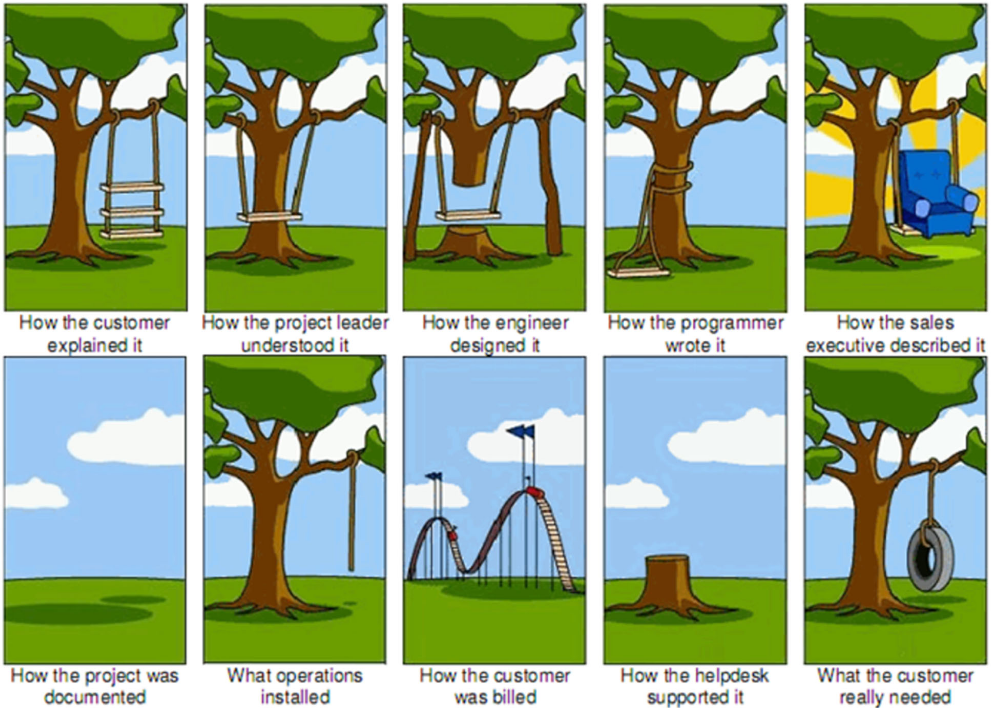
\includegraphics[height=3.4in]{figs2/tree-swing-requirements-issue.png}
	\end{center}
\end{figure}

\vspace{10pt}

\subsubsection{Job and Role Titles}
There is no consensus across private or public industries regarding the titles used for CS job roles. Terms such as developer, programmer, software engineer, designer, analyst, and architect, are often used as the titles for CS job postings. However, the job duties and desired skills listed for these positions will vary widely. When considering CS job opportunities, it is best to look past the position title and use the skills and responsibilities to understand what the job entails.

\subsubsection{Common CS Project Roles}
Figure \ref{fig:figure2} depicts many roles involved in creating a CS-based product, comparing how much business versus CS expertise a person needs for the role. These relative comparisons are not absolutes, and different team members will have a mix of skills. Table \ref{tab:table2} describes the roles depicted in Figure \ref{fig:figure2}. The arrangement of the table does not represent a management reporting structure. Often, a person's manager is not someone they work with daily; instead, they work with their product team(s), and their manager is there to provide support within the organization, such as career planning, advancement, and training. 

\begin{figure}[H]
	\begin{center}
		\caption{Product Team Roles Mapped to CS and Domain Knowledge}
		\label{fig:figure2}
		\vskip 4pt
		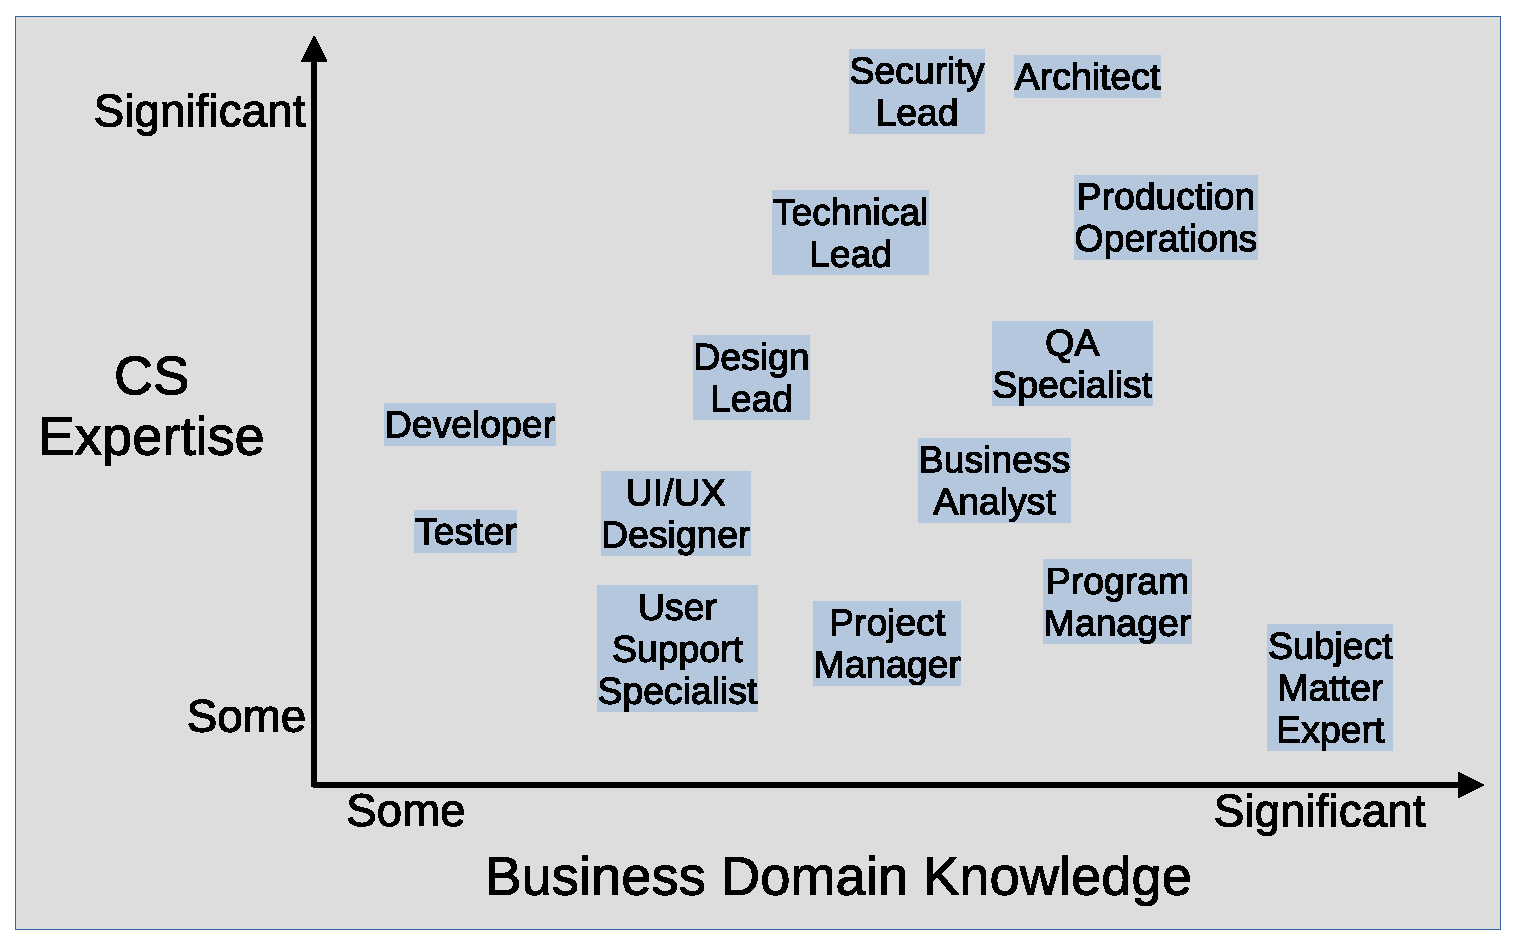
\includegraphics[height=2.9in]{figs2/cs-team-roles-knowledge-area.eps}
	\end{center}
\end{figure}


%\begin{center}

\index{program manager}
\index{product manager}
\index{ui/ux design}
\index{ux design}
\index{architect}
\index{security lead}
\index{technical lead}
\index{business analyst}
\index{BA}
\index{developer}
\index{tester}
\index{quality assurance}
\index{QA}
\index{production operations}
\index{subject matter expert}
\index{SME}
\index{user support specialist}
\index{CS team role!program manager}
\index{CS team role!product manager}
\index{CS team role!ui/ux design}
\index{CS team role!ux design}
\index{CS team role!architect}
\index{CS team role!security lead}
\index{CS team role!technical lead}
\index{CS team role!business analyst}
\index{CS team role!BA}
\index{CS team role!developer}
\index{CS team role!tester}
\index{CS team role!quality assurance}
\index{CS team role!QA}
\index{CS team role!production operations}
\index{CS team role!subject matter expert}
\index{CS team role!SME}
\index{CS team role!user support specialist}

\begin{longtable}[H]{p{.8in}|p{3.6in}}
	\caption{CS-related Team Roles}
	\label{tab:table2}\\
	\textbf{Role} & \textbf{Description}\\
	\hline
	\endfirsthead
	\textbf{Role} & \textbf{Description}\\
	\endhead
	\Tstrut Program Manager & Manages multiple products. Assures teams have the resources and people they need, clarifies to team members how the products fit into the organization's goals and objectives and coordinates requirements and schedules with internal and external stakeholders.\\
	\hline
	\Tstrut Product Manager & Manages the creation and maintenance of a product. Coordinates schedules across team members, assures team has the resources and people needed to succeed, clarifies ambiguities in priorities for features, communicates status information to stakeholders.\\
	\hline
	\Tstrut UI/UX \linebreak Designer & Responsible for user experience and user interface design. They assess how people will interact with the product, including considering accessibility, such as how those who are visually or auditorially impaired, color blind, or unable to control an interface with a mouse or standard keyboard will use the product. They also consider the application's aesthetics, using colors, fonts, and positions of controls, physical and on-screen, to create a pleasant and coherent interface for the user.\\
	\hline
	\Tstrut Architect & Designs the infrastructure for the product. Most computer-based products involve multiple types of technology that have to be linked together. These technologies, such as databases, web services, user interfaces, authentication and authorization (login and permissions), and document management (images, videos, audio), can be used differently. The architect defines how the product teams will use these technologies. They also ensure the products continue working well when user load increases, known as load balancing, or when a piece of hardware fails, known as failover.\\
	\hline
	\Tstrut Security Lead & Responsible for the security aspects of the product. Protecting user data requires careful design of the product's hardware and software. This person understands the threats to the product and its data and works with the team to design mitigations to thwart attackers. Security is a broad area in an organization, including physical and virtual security, and many companies have security teams with individuals responsible for identifying and handling different types of breaches.\\
	\hline
	\Tstrut Technical Lead & Responsible for the overall technical design of the product. The role is sometimes referred to as the design lead. These team members manage decisions about programming languages, third-party packages, data structures, algorithms, and test integrations. This individual has worked as a developer and gained experience with multiple programming languages, packages, development tools, and platforms.\\
	\hline
	\Tstrut Business Analyst & The business analyst (BA) is responsible for understanding and communicating the requirements for the product. This individual is the bridge between the business and computer science experts. BAs must understand the business objectives for the product and have some experience with CS concepts, such as basic programming, data structures, and testing. BAs are the "voice of the customer," assuring the team remains focused on creating a product that meets the organization's and users' needs.\\
	\hline
	\Tstrut Developer & Responsible for writing the programs required for the product. Developers have expertise in one or more programming languages and third-party packages or libraries. Developers may specialize in back-end, mid-tier, front-end, and full-stack development. The back-end involves accessing and storing data, including securing the information. Mid-tier development focuses on sending information between systems, often as web services. Front-end developers focus on the user interface, whether using graphical development environments for smartphones and computers or web technologies such as HTML and CSS for web browsers. Full-stack developers have experience and expertise throughout all application tiers. \\
	\hline
	\Tstrut Tester & Responsible for unit and integration testing of the programs used in the product. The individual is familiar with testing and mocking frameworks and performance and load-testing tools. They play a vital role in assuring that the code created by the developer does what it is supposed to do and does not do things it should not, such as failing to properly handle an unexpected input value.\\
	\hline
	\Tstrut QA \linebreak Specialist & The quality assurance (QA) team is responsible for verifying the entire product's quality. This verification requires testing the completed product to be sure it does everything the product owner requested and that the BAs documented. It also means verifying that the product comprehensively protects users and their information from harm or misuse, such as loss or corruption of data. The QA function in an organization often operates in an environment that matches that of the final production environment but is specifically designed to record, playback, and verify the operations of the product using automation tools. QA is also responsible for verifying that the product will work under anticipated conditions, such as a large number of users using the product simultaneously or being able to failover to a backup site if a natural disaster strikes.\\
	\hline
	\Tstrut Production Operations  & The production team is responsible for the ongoing operation of the product once QA has approved it. The production team manages the organization's infrastructure, including servers, networks, backup power supplies, physical security of equipment, user accounts, and Internet access. The team includes people knowledgeable in operating systems, networking protocols, application configuration, database management, physical security, and help desk services. These individuals keep systems functioning and help users when problems arise.\\
	\hline
	\Tstrut Subject \linebreak Matter \linebreak Expert & A subject matter expert (SME) is an expert in the business or field that makes up the focus of the product. For healthcare companies, SMEs are doctors and nurses; at legal companies, they are lawyers and paralegals; for tax and finance companies, they are accountants and banking experts. An SME provides detailed information about how the product must work and can answer questions about its features and operations. The SME, BA, and QA often work closely to ensure the final product meets users' needs.\\
	\hline
	\Tstrut User \linebreak Support \linebreak Specialist & User support specialists have several responsibilities. They create documentation for users, train users, and provide scripts for the help desk to use when a problem arises. In this role, the individual works with the BA, development team, and QA, to ensure documentation is accurate and meets the user's needs. In their role as trainers, they are often the face of the product for users, becoming a trusted resource when a user has additional questions.\\ 
	\bottomrule
\end{longtable}

%\end{center}

After considering all these roles, you may see that computer science is a broad field with opportunities for people of many different backgrounds to combine their talents to create unique products. Whether a new smartphone game app or an advanced surgical robot, CS expertise is a critical component many organizations need to create their products. What makes CS interesting is that as someone gains experience, they can choose different career paths, some preferring to become more technical and others finding more reward in business-centric and user-focused roles.

An important point to note is that programming, primarily the developer's domain, represents a small part of the team and overall effort of implementing a computer-based product. People often equate CS and programming, believing there is little else to CS than writing code; however, that is not the case. Programming is integral to creating a computer-based product, but it only represents some of the work.

\newpage

\index{CS careers}
\index{careers!CS}

\section{A Survey of CS-related Careers}
\index{CS-related Careers}
\index{Careers involving in CS}
\index{Jobs involving in CS}

We have provided this section to give you an idea of the breadth of work that intersects with CS. It is a survey touching on a few examples across different specialties, and the descriptions are purposefully brief. You can always follow up with your instructor or do online research if a role sounds interesting.

\subsection{Arts and Media}

\index{arts and media technology careers}
\index{technology careers!arts and media}
\index{film and video editing}
\index{multimedia art and animation}
\index{video game design}
\index{web design}

\begin{figure}[H]
	\begin{center}
		\caption{Video Editing}
		\vskip 4pt
		
\includegraphics[height=2in]{images/careers/iStock-922654000.small.jpg}
	\end{center}
\end{figure}

\begin{table}[H]
	\begin{center}
		\caption{Arts and Media Technology Careers}
		\vskip 4pt
		\begin{tabular}{p{1in}|p{3.4in}} 
			\textbf{Role} & \textbf{Description}\\
			\hline
			Film and video editing & Editors work with directors and producers to pull together all aspects, such as video, animation, special effects, sound effects, soundtracks, and dialog, of the movie or show. Editors use specialized hardware and software to complete the editing work.\\
			\hline
			Multimedia art and animation & Whether special effects in movies or the virtual worlds of immersive games, multimedia artists use their artistic skills and knowledge of animation and drawing software to bring their ideas to life.\\
			\hline
			Video game design & Video game design overlaps with movie making. Games need plots, game elements, animation, dialog, soundtracks, and much more. Game designers combine these elements using different software packages and libraries to create content and implement the game's logic.\\
			\hline
			Web design & Developing appealing, useful, and responsive websites is a creative endeavor bringing together visual and technical design. There are many frameworks and languages that website developers choose from based on their needs, time frame, and budget.\\
			\hline
		\end{tabular}
	\end{center}
\end{table}

\subsection{Data}

\index{data technology careers}
\index{technology careers!data}
\index{data analysis}
\index{data science}
\index{data wrangling}
\index{database administration}

\begin{figure}[H]
	\begin{center}
		\caption{Data Analysis}
		\vskip 4pt
		
\includegraphics[height=2in]{images/careers/iStock-1364769258.small.jpg}
	\end{center}
\end{figure}

\begin{table}[H]
	\begin{center}
		\caption{Data Careers}
		\vskip 4pt
		\begin{tabular}{p{1in}|p{3.4in}} 
			\textbf{Role} & \textbf{Description}\\
			\hline
			Data analysis & Involves summarizing and connecting the data in ways that help business leaders identify risks and opportunities in their operations and markets. The work often involves finding novel visualizations to make the information apparent.\\
			\hline
			Data science & This is a broad term for work that involves manipulating, summarizing, or identifying patterns in data. Data science includes data mining, machine learning, and AI.\\
			\hline
			Data wrangling & Although data analysis and data science get much attention, these roles need high-quality, curated data. Those adept at data wrangling manipulate data from different sources, identify and fix quality issues, and combine related information to create unbiased and well-defined data sets for analysis and mining.\\
			\hline
			Database\linebreak administration & The volume, velocity, veracity, and variability in data make its management complex. At the broadest level, digital data exists in structured and unstructured forms. Database administration involves the storage, retrieval, organization, and protection of a constantly-growing collection of data, making sure it is available for efficient access, but only to those authorized to access it.\\
			\hline
		\end{tabular}
	\end{center}
\end{table}

\subsection{Data Security}

\index{data security technology careers}
\index{technology careers!data security}
\index{blue team}
\index{honeypot administration}
\index{pen tester}
\index{penetration testing}
\index{red team}

\begin{figure}[H]
	\begin{center}
		\caption{Blue team}
		\vskip 4pt
		
\includegraphics[height=2in]{images/careers/iStock-949581032.small.jpg}
	\end{center}
\end{figure}

\begin{table}[H]
	\begin{center}
		\caption{Data Security Careers}
		\vskip 4pt
		\begin{tabular}{p{1in}|p{3.4in}} 
			\textbf{Role} & \textbf{Description}\\
			\hline
			Blue team & This team identifies, stops, and mitigates the efforts of people attacking a company's systems. This team develops plans for handling attacks, works with law enforcement if a breach occurs, and takes the lead in handling active attacks. They are the flip side of the Red Team (see: Red team).\\
			\hline
			Honeypot\linebreak administration & A honeypot is a computer with no business purpose other than to attract and detect attackers. Those operating honeypots seek to make the system look like a real business system and then carefully record the actions of those who access it, knowing they are attackers. Honeypots are a powerful tool for finding insider and outsider threats to an organization.\\
			\hline
			Pen testing & Companies hire pen testers to breach their organization's systems. This work might include getting past physical security barriers and breaking into computers over a network. Pen testing is a popular way for companies to assess the quality of their cyber defenses.\\
			\hline
			Red team & This team is an adversary to the Blue team (see: Blue team). This team takes actions that an attacker would take to identify weaknesses in defenses and allow the Blue team to test their procedures. Blue and red team members often rotate between teams to broaden their security skills.\\
			\hline
		\end{tabular}
	\end{center}
\end{table}


\subsection{Education}

\index{education technology careers}
\index{technology careers!education}
\index{educational content creation}
\index{content creation!education}
\index{educational software design}
\index{teaching}
\index{training}

\begin{figure}[H]
	\begin{center}
		\caption{Educational Software}
		\vskip 4pt
		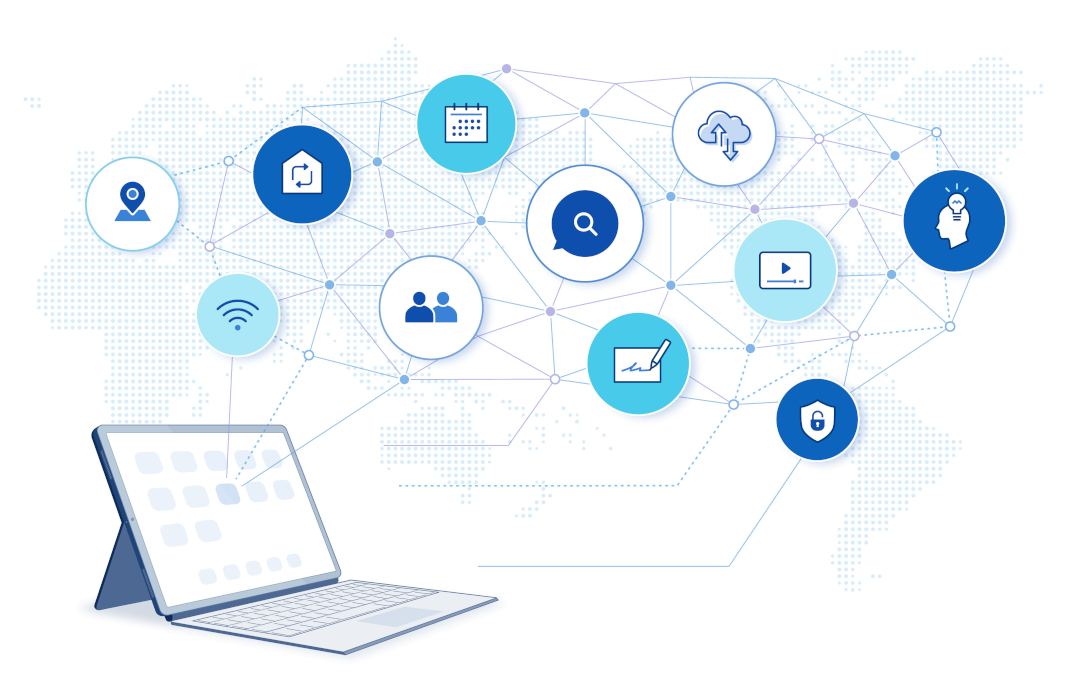
\includegraphics[height=2in]{images/careers/iStock-1360633055.small.jpg}
	\end{center}
\end{figure}

\begin{table}[H]
	\begin{center}
		\caption{Educational Technology Careers}
		\vskip 4pt
		\begin{tabular}{p{1in}|p{3.4in}} 
			\textbf{Role} & \textbf{Description}\\
			\hline
			Content\linebreak creation & Online education, and flipped classrooms require digital educational materials. Content creators are knowledgeable in their fields, whether cooking, biology, music or many other subjects. They also consider how to keep online students engaged using gamification techniques, well-designed graphics, and interactive exercises. Teams work to create an engaging, thought-provoking, and immersive learning environment that adjusts to the learner's needs.\\
			\hline
			Educational software design & To deliver educational content online effectively, specialized software is needed. The programs include platforms for learning, document, and workflow management. These tools are often developed as web-based environments with additional features for mobile devices.\\
			\hline
			Teaching and training & The foundation of education are teachers and students. As students become more tech-savvy, teachers' platforms and approaches must keep pace. Finding ways to combine effective pedagogical and andragogical techniques with technology can create a more rewarding experience for the instructor and lead to more effective learning by the student. Teaching is not limited to schools; many businesses have trainers who train employees on internal tools and procedures or train customers to teach them how to use the company's products.\\
			\hline
		\end{tabular}
	\end{center}
\end{table}

\subsection{Finance and Insurance}

\index{finance technology careers}
\index{technology careers!finance}
\index{insurance technology careers}
\index{technology careers!insurance}
\index{credit and portfolio analysis}
\index{investment banking}
\index{financial planning}
\index{risk analysis}

\begin{figure}[H]
	\begin{center}
		\caption{Risk Analysis}
		\vskip 4pt
		
\includegraphics[height=2in]{images/careers/iStock-1210565724.small.jpg}
	\end{center}
\end{figure}

\begin{table}[H]
	\begin{center}
		\caption{Finance Technology Careers}
		\vskip 4pt
		\begin{tabular}{p{1in}|p{3.4in}} 
			\textbf{Role} & \textbf{Description}\\
			\hline
			Credit and\linebreak portfolio analysis & Companies of all kinds utilize many data-centric metrics to assess their financial health and identify issues they must address. Producing accurate and timely metrics requires significant data processing, statistical, and financial expertise. Organizations define Key Performance Indicators (KPIs) to monitor their operations, each requiring the integration and synthesis of data.\\
			\hline
			Investment banking & Identifying good investments, and keeping track of investment performance are vital for many financial institutions. Larger institutions coordinating significant financial events, such as mergers and acquisitions, rely on data analysis and modeling to recognize good investment opportunities.\\
			\hline
			Financial\linebreak planning & Working with individuals and organizations to plan for future financial needs is rewarding. Financial planners utilize a variety of data sources and data modeling tools, coordinating with the goals of each customer to identify optimal investment strategies.\\
			\hline
			Risk analysis & Companies assess risk for many reasons. For example, insurance companies make their money by properly modeling the financial risk presented by the insured. Insurance exists in many domains, such as healthcare, property and casualty, automobile, and insurance company portfolios. Utilizing data analysis, modeling, and machine learning, insurance companies design their offerings to be affordable and ensure they can pay the claims for losses suffered by their customers.\\
			\hline
		\end{tabular}
	\end{center}
\end{table}

\subsection{Government}

\index{government technology careers}
\index{technology careers!government}
\index{cryptographic analysis}
\index{cyber terrorism defense}
\index{vulnerability discovery}
\index{pharmacy benefits administration}

\begin{figure}[H]
	\begin{center}
		\caption{Cyber Terrorism Defense}
		\vskip 4pt
		
\includegraphics[height=2in]{images/careers/iStock-1169668290.small.jpg}
	\end{center}
\end{figure}

\begin{table}[H]
	\begin{center}
		\caption{Government Technology Careers}
		\vskip 4pt
		\begin{tabular}{p{1in}|p{3.4in}} 
			\textbf{Role} & \textbf{Description}\\
			\hline
			Cryptographic analysis & Cryptography is an active area of research. It serves as the basis for securing data stored in a system or accessed across the Internet. Attackers and ever more powerful computers consistently drive the need for new and more effective ways to secure information. This field involves math and creativity. There are no formal proofs of a cryptographically secure algorithm, and careers in cryptography range from creating new cryptographic approaches to finding weaknesses in existing or proposed algorithms.\\
			\hline
			Cyber terrorism defense & Governments and companies find themselves targeted by cyber attackers and terrorists. To protect themselves and those who use their services, they maintain teams of cyber experts to defend their systems. These include blue teams (see: Data Security: Blue team), those with military experience, and others with deep knowledge of application and network protocols.\\
			\hline
			Vulnerability discovery & Similar to pen testing (see: Data Security: Pen tester), teams working in vulnerability discovery seek to identify and remediate weaknesses in an organization's infrastructure. These teams often work with software development teams and guide them to strengthen the security of the application the team is building. They also work with QA to design effective security-focused tests. In some cases, governments will scan and proactively alert companies to vulnerabilities to thwart attackers.\\
			\hline
		\end{tabular}
	\end{center}
\end{table}

\subsection{Healthcare}

\index{healthcare technology careers}
\index{technology careers!healthcare}
\index{clinical informatics}
\index{medical outcomes analysis}
\index{outcomes analysis!medical}
\index{medical coding and billing}

\begin{figure}[H]
	\begin{center}
		\caption{Clinical Informatics}
		\vskip 4pt
		
\includegraphics[height=2in]{images/careers/iStock-1189303763.small.jpg}
	\end{center}
\end{figure}

\begin{table}[H]
	\begin{center}
		\caption{Healthcare Technology Careers}
		\vskip 4pt
		\begin{tabular}{p{1in}|p{3.4in}} 
			\textbf{Role} & \textbf{Description}\\
			\hline
			Clinical\linebreak informatics & Takes data from medical devices, patient record systems, pharmaceutical databases, and genetics research to identify and treat health issues. Teams involve experts in all aspects of healthcare and computer science. Large datasets are combined, analyzed, modeled, and assessed. These roles exist in healthcare companies, hospitals, doctors' offices, research institutions, and companies that serve those fields.\\
			\hline
			Outcomes\linebreak analysis & A vital part of improving healthcare is identifying good versus poor treatment outcomes. The work can also involve looking at recent trends to identify changes to environments or other factors that require adjusting treatment protocols quickly.\\
			\hline
			Medical coding and billing & Healthcare payers (insurance companies) utilize healthcare data in interesting ways. One area of particular interest is identifying healthcare fraud, which does more harm than just wasting money; it diverts funding from those who need it. Using data analysis and machine learning, billing teams find erroneous or unusual diagnoses or treatment patterns.\\
			\hline
			Pharmacy\linebreak benefits administration & Assuring patients get the drugs they need without undue risk due to drug interactions involves the integration of patient databases, pharmaceutical data, genetic data, and insurance records. Identifying dangerous drug interactions goes beyond mapping drugs that interact to consider prior diseases the patient has had and their genetic makeup.\\
			\hline
		\end{tabular}
	\end{center}
\end{table}

\subsection{Logistics/Transportation}

\index{logistics technology careers}
\index{technology careers!logistics}
\index{transportation technology careers}
\index{technology careers!transportation}
\index{blockchain integration}
\index{self-driving vehicles}
\index{supply chain management}

\begin{figure}[H]
	\begin{center}
		\caption{Supply Chain Management}
		\vskip 4pt
		
\includegraphics[height=2in]{images/careers/iStock-1399747292.small.jpg}
	\end{center}
\end{figure}

\begin{table}[H]
	\begin{center}
		\caption{Logistics Technology Careers}
		\vskip 4pt
		\begin{tabular}{p{1in}|p{3.4in}} 
			\textbf{Role} & \textbf{Description}\\
			\hline
			Blockchain\linebreak integration & Blockchain technology allows companies to share a database whose transactions are secured using cryptography. Although often conflated with cryptocurrencies, blockchain is an approach to a decentralized database that companies can use to track the supply and movement of goods and services. Those with blockchain expertise often work with product development teams to integrate a blockchain into the platform.\\
			\hline
			Self-driving vehicles & The development of autonomous vehicles rely on AI techniques, including machine learning. It is infeasible to program a car or truck manually; it must be able to recognize, respond, and adapt to different conditions. Due to an ongoing shortage of qualified drivers, the trucking industry is actively pursuing self-driving trucks, particularly to handle the "long haul" (highway) aspects of trucking.\\
			\hline
			Supply chain management & Coordinating the production and movement of goods in a global economy involve processing data from many different companies, including manufacturing, shipping, and retail. Each company has unique systems and data formats, complicating things further. Skills in data management, data wrangling, and data analysis are consistently in demand, as are team members for companies building applications that coordinate supply chains between organizations.\\
			\hline
		\end{tabular}
	\end{center}
\end{table}

\subsection{Machine Learning}

\index{machine learning careers}
\index{technology careers!machine learning}
\index{artificial intelligence}
\index{AI}
\index{data mining}
\index{operations research}
\index{virtual reality}
\index{VR}

\begin{figure}[H]
	\begin{center}
		\caption{Virtual Reality}
		\vskip 4pt
		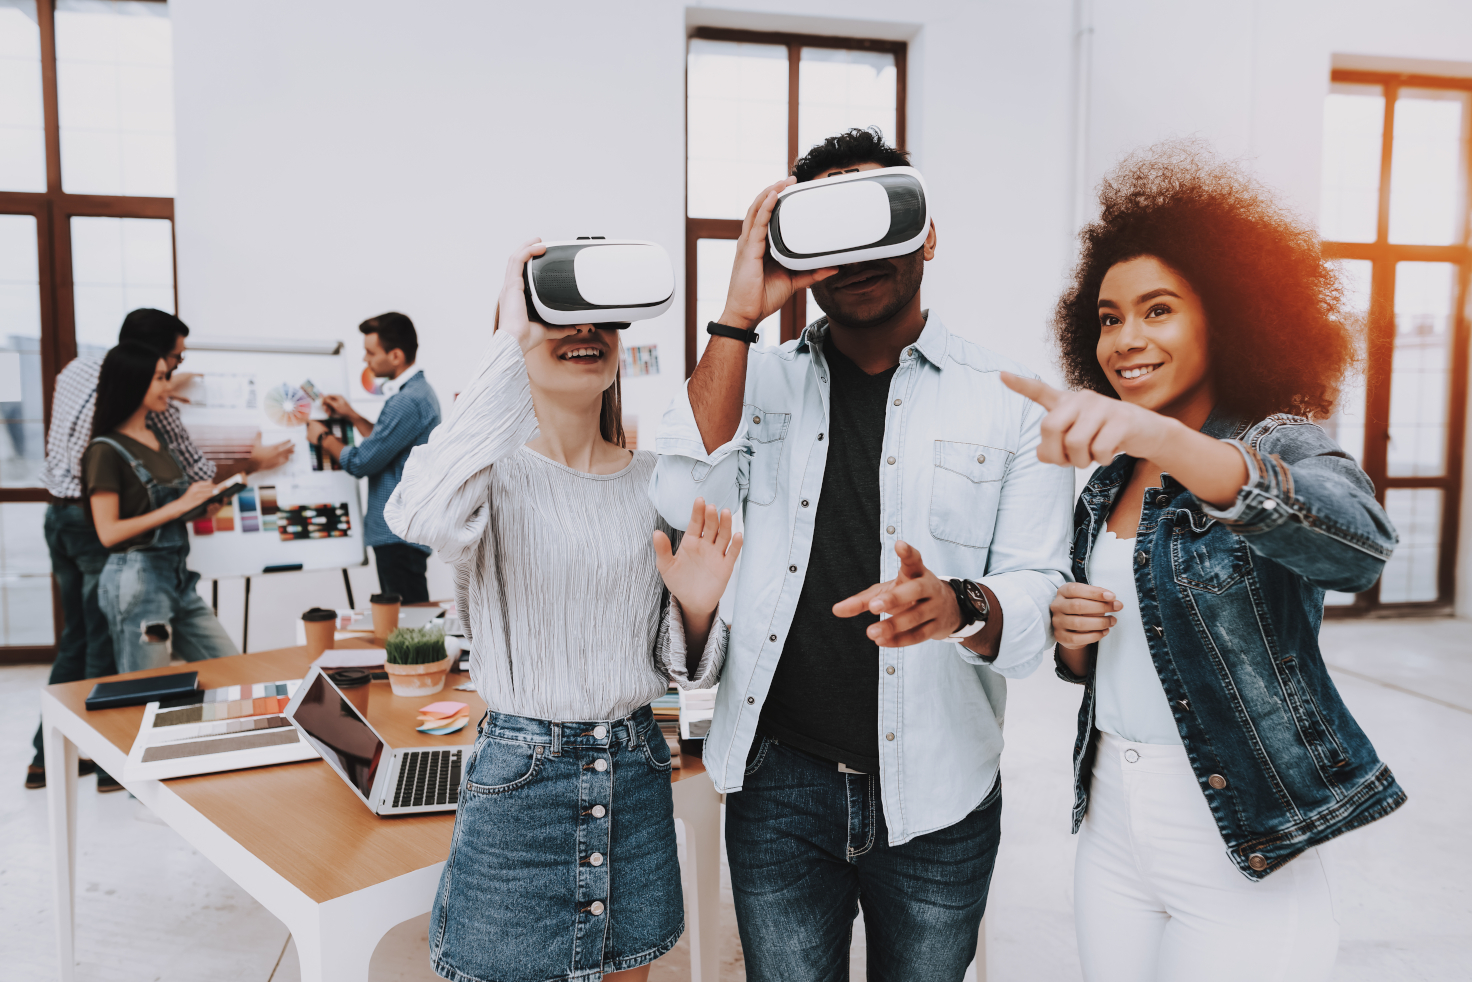
\includegraphics[height=2in]{images/careers/iStock-1051052494.small.jpg}
	\end{center}
\end{figure}

\begin{table}[H]
	\begin{center}
		\caption{Machine Learning Careers}
		\vskip 4pt
		\begin{tabular}{p{1in}|p{3.4in}} 
			\textbf{Role} & \textbf{Description}\\
			\hline
			Artificial\linebreak intelligence & AI is a catch-all term for systems that demonstrate intelligence, meaning they can solve problems independently. Much of AI currently relies on machine learning, but AI is broader than that. Numerous roles are related to AI, including algorithmic research, computer hardware, specialized sensors, and software. AI can automate many existing technologies, such as robots, online support centers, and diagnostic services.\\
			\hline
			Data mining & This field is used in most industries to identify opportunities from their data. Unlike many other uses of machine learning, data miners may not know what they are looking for; rather, they explore the data to see if there is a model to find.\\
			\hline
			Operations\linebreak research & Those working in this field use data analytics and data mining to model different scenarios. Their goal is to identify the optimum strategies or solutions to problems posed by an organization. Many organizations have teams providing this service, including government departments and larger corporations.\\
			\hline
			Virtual reality (VR) & The VR field has gone from a gamer-focused technology to broader applications, including psychological research and treatment, architecture and construction, and medical training. VR teams consist of SMEs in different fields, such as psychology, and those skilled in software development and the visual arts.\\
			\hline
		\end{tabular}
	\end{center}
\end{table}

\subsection{Manufacturing and Utilities}

\index{manufacturing technology careers}
\index{technology careers!manufacturing}
\index{utilities technology careers}
\index{technology careers!utilities}
\index{enterprise resource planning}
\index{ERP}
\index{industrial automation}
\index{robotics}

\begin{figure}[H]
	\begin{center}
		\caption{Robotics}
		\vskip 4pt
		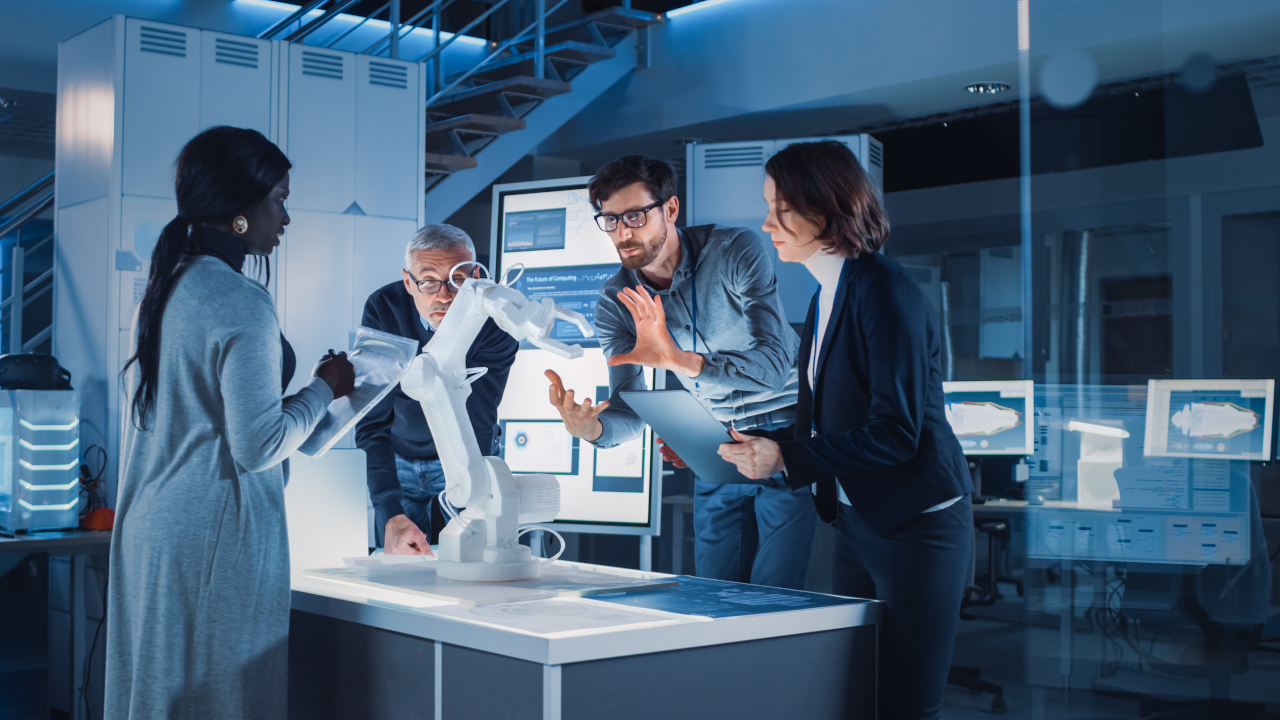
\includegraphics[height=2in]{images/careers/iStock-1214111404.small.jpg}
	\end{center}
\end{figure}

\begin{table}[H]
	\begin{center}
		\caption{Manufacturing and Utilities Technology Careers}
		\vskip 4pt
		\begin{tabular}{p{1in}|p{3.4in}} 
			\textbf{Role} & \textbf{Description}\\
			\hline
			Enterprise\linebreak resource\linebreak planning & Enterprise resource planning (ERP) is a complex task that combines data from engineers, industrial designers, manufacturing SMEs, robotic systems, customers, and suppliers to map out the scheduling of production work across a factory. The popularity of just-in-time (JIT) manufacturing adds to the complexity of the effort, which involves data analysis, specialized planning, and operating software.\\
			\hline
			Industrial\linebreak automation & Utility and infrastructure organizations, such as power generation and subways, utilize specialized computer hardware and software, known as supervisory control and data acquisition (SCADA) systems, to monitor and control their equipment. Many organizations connect SCADA systems to the Internet for remote access, yet these systems were designed decades ago, predating computer networking with no consideration of data security. There is widespread concern about attackers disabling power or transit systems through Internet attacks leading to increased demand for people with expertise in configuring and protecting these systems.\\
			\hline
			Robotics & Many aspects of manufacturing involve automated processes. These systems require specific instructions and data to perform the correct actions at the right time. As companies fabricate new items or change the materials used to build a part, the systems managing the process need to change. This field utilizes a wide variety of specialized hardware and software.\\
			\hline
		\end{tabular}
	\end{center}
\end{table}

\subsection{Music and Entertainment}

\index{music technology careers}
\index{technology careers!music}
\index{entertainment technology careers}
\index{technology careers!entertainment}
\index{musical arranging}
\index{sound engineering}
\index{sound recording}
\index{sound mixing}
\index{arranging!musical}
\index{engineering!sound}
\index{recording!sound}
\index{mixing!sound}
\index{performance!technology in}

\begin{figure}[H]
	\begin{center}
		\caption{Editing and Mixing}
		\vskip 4pt
		
\includegraphics[height=2in]{images/careers/iStock-1176082646.small.jpg}
	\end{center}
\end{figure}

\begin{table}[H]
	\begin{center}
		\caption{Music and Performance Technology Careers}
		\vskip 4pt
		\begin{tabular}{p{1in}|p{3.4in}} 
			\textbf{Role} & \textbf{Description}\\
			\hline
			Arranging & Often, an artist works with an arranger to take the music they have written and work out the instrumentation used in its performance. Music notation and musical instrument digital interface (MIDI) systems play a prominent role in this work. Artists and arrangers can use musical notation on a computer to control digital instruments and hear the result immediately. Even if the final performance will be on non-digital instruments, this approach speeds the process.\\
			\hline
			Engineering, recording,\linebreak and mixing & Music recording involves combining and balancing many input sources. These inputs are the sounds from singers and instrumentalists, stored as computer data. Sound engineers shape the tonal experience for the listener, sometimes bringing together hundreds of individual sound sources. Engineers use soundboards that match the ergonomics of analog equipment, but control computer systems that mix and store the audio data.\\
			\hline
			Performance & Many artists include digital instruments in their ensemble and use MIDI to run aspects of their performance and coordinate an array of special effects. Far beyond the music itself, integrating musical instruments and other aspects of a show, such as lighting and specialized video, requires the work of visual artists, audio engineers, electricians, and developers with expertise in programming the specialized systems used to interface and coordinate data between these devices.\\
			\hline
		\end{tabular}
	\end{center}
\end{table}

\subsection{Research}

\index{research technology careers}
\index{technology careers!research}
\index{medical device research}
\index{modeling}

\begin{figure}[H]
	\begin{center}
		\caption{Agriculture Modeling and Management}
		\vskip 4pt
		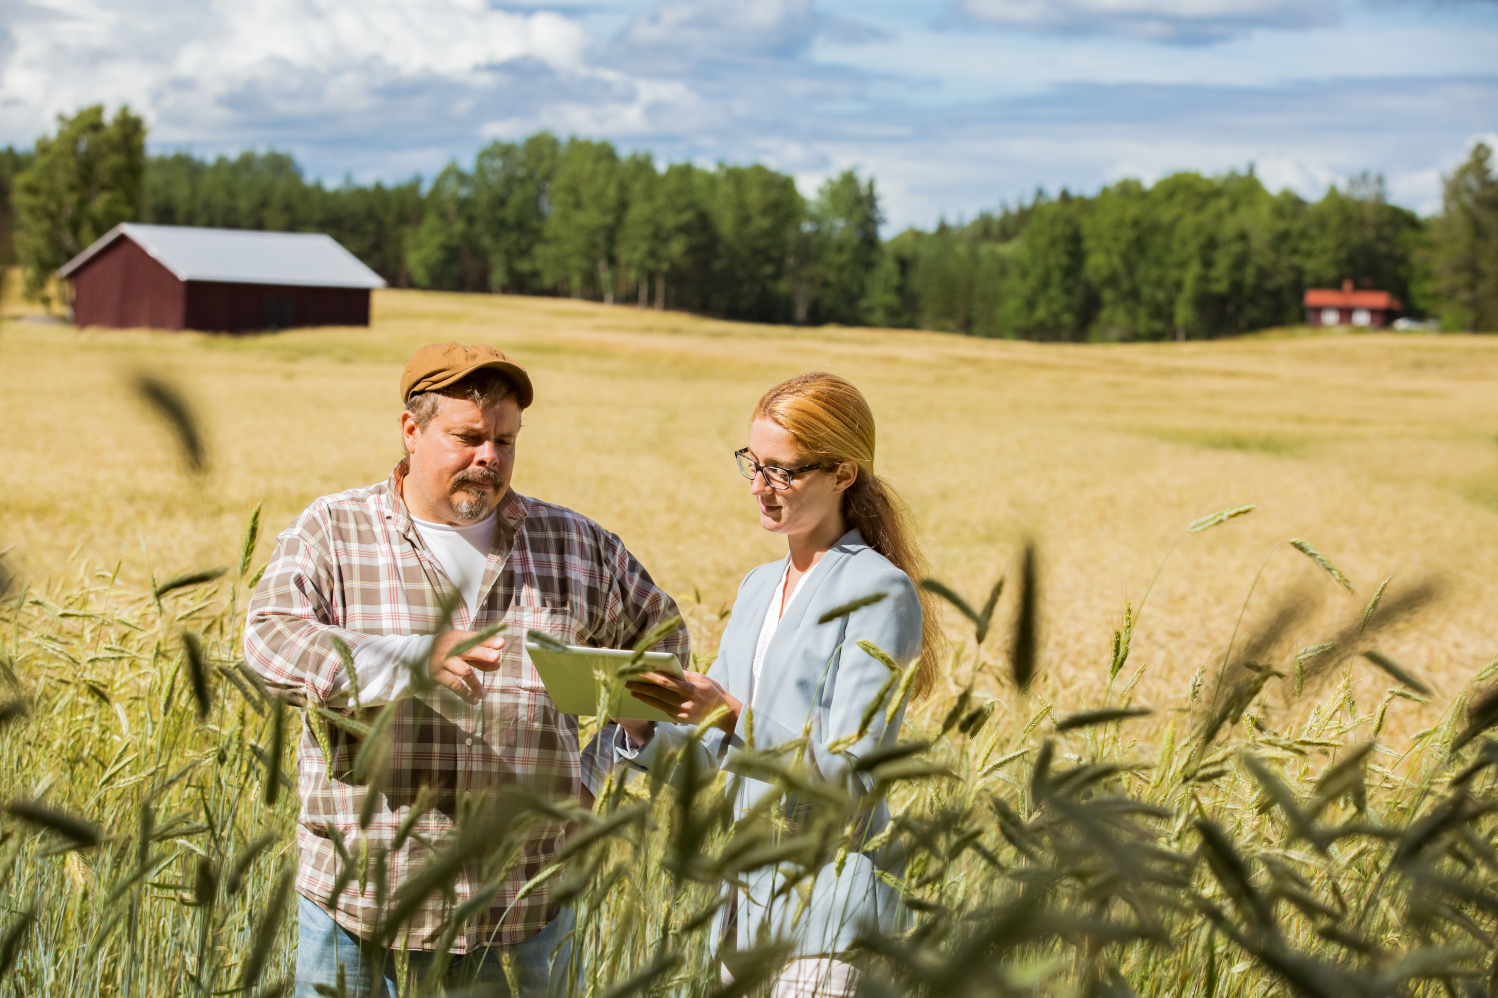
\includegraphics[height=2in]{images/careers/iStock-1272791496.small.jpg}
	\end{center}
\end{figure}

\begin{table}[H]
	\begin{center}
		\caption{Research Technology Careers}
		\vskip 4pt
		\begin{tabular}{p{1in}|p{3.4in}} 
			\textbf{Role} & \textbf{Description}\\
			\hline
			Medical device research & The pace of change in medicine continues to accelerate. Nanotechnology, wearables, robotic surgery, and WiFi-enabled implants offer an expansive world of possibilities for detecting and treating many health conditions. Teams include doctors, nurses, hardware specialists, data analysis, and software development teams to develop, test, and operationalize these devices. The work is not limited to the device's functions; teams create applications to control, record, analyze, and respond to the device's output. Further, specialized training for medical personnel and patients must be created and presented. Being healthcare-related, teams must account for security and privacy to prevent unintended changes to the device's operation and to protect patient privacy.\\
			\hline
			Modeling & Modeling provides tools to evaluate different options, test multiple hypotheses, and seek optimum solutions in many fields, such as agriculture, biodiversity, climate change, ecology, water management, and waste management. There are many opportunities to combine the expert knowledge of SMEs and information from satellites, weather stations, and specialized sensors, using data science techniques to understand and begin to manage significant challenges in our world.\\
			\hline
		\end{tabular}
	\end{center}
\end{table}

\newpage

\section{Exercises}

\begin{ex}
	Look up Moore's Law and explain the concept Moore described and its implications on computers and other electronic devices. Where have you seen evidence of this?	
\end{ex}

\begin{ex}
	Look up the term "information economy." Define and explain it in your own words. Consider a career or field that interests you and find or suggest ways computers impact or might impact the work done in that field.
\end{ex}

\begin{ex}
	Create a table listing all the computing devices and programs (software) you have come into contact with in the last month, their purposes, and the total time you have interacted with them during the month. Expand your list to include other computing devices and programs and their purposes; these might be devices or software you have come into contact with in the past or that you are aware of in other ways (e.g., heard about from others, saw on a news show). Each device and program required teams of analysts, designers, developers, testers, trainers, and production engineers to bring them to fruition. Choose the top three that you would have found interesting to work on and consider which team role(s) you would have found most rewarding.
	 
\end{ex}

\begin{ex}\label{exCh18Timeline}
	Extend the CS timeline found in Appendix \ref{appendixTimeline} on page \pageref{appendixTimeline} to add more CS milestones, particularly after 2011, that you find interesting or noteworthy.
\end{ex}